\section{Deep Q-Learning (Neural Network as Q-Function)}
\subsection{Architecture}\label{sec:arch}
\begin{enumerate}

\item For the Q-function, we use a Neural Network network with $2$ hidden layer of $32$ units each. The output layer has $5$ outputs , one corresponding to each action.
\item For the \texttt{discrete} case there are total 
$\texttt{n}_{\texttt{speed}} \times \texttt{n}_{\texttt{lanes}} \times  \texttt{n}_{\texttt{dist}}^{\texttt{n}_{\texttt{lanes}}} = 10,000$  states and we use embeddings of size $16$.
\item For the \texttt{discrete} case there are total 
$\texttt{n}_{\texttt{speed}} \times \texttt{n}_{\texttt{lanes}} = 16$ states and we use embeddings of size $4$. The distances $d_1, d_2, d_3, d_4$ are directly concatenated.
\end{enumerate}

\begin{figure}[H]
    \centering
    \begin{minipage}{0.49\linewidth}
        \centering
        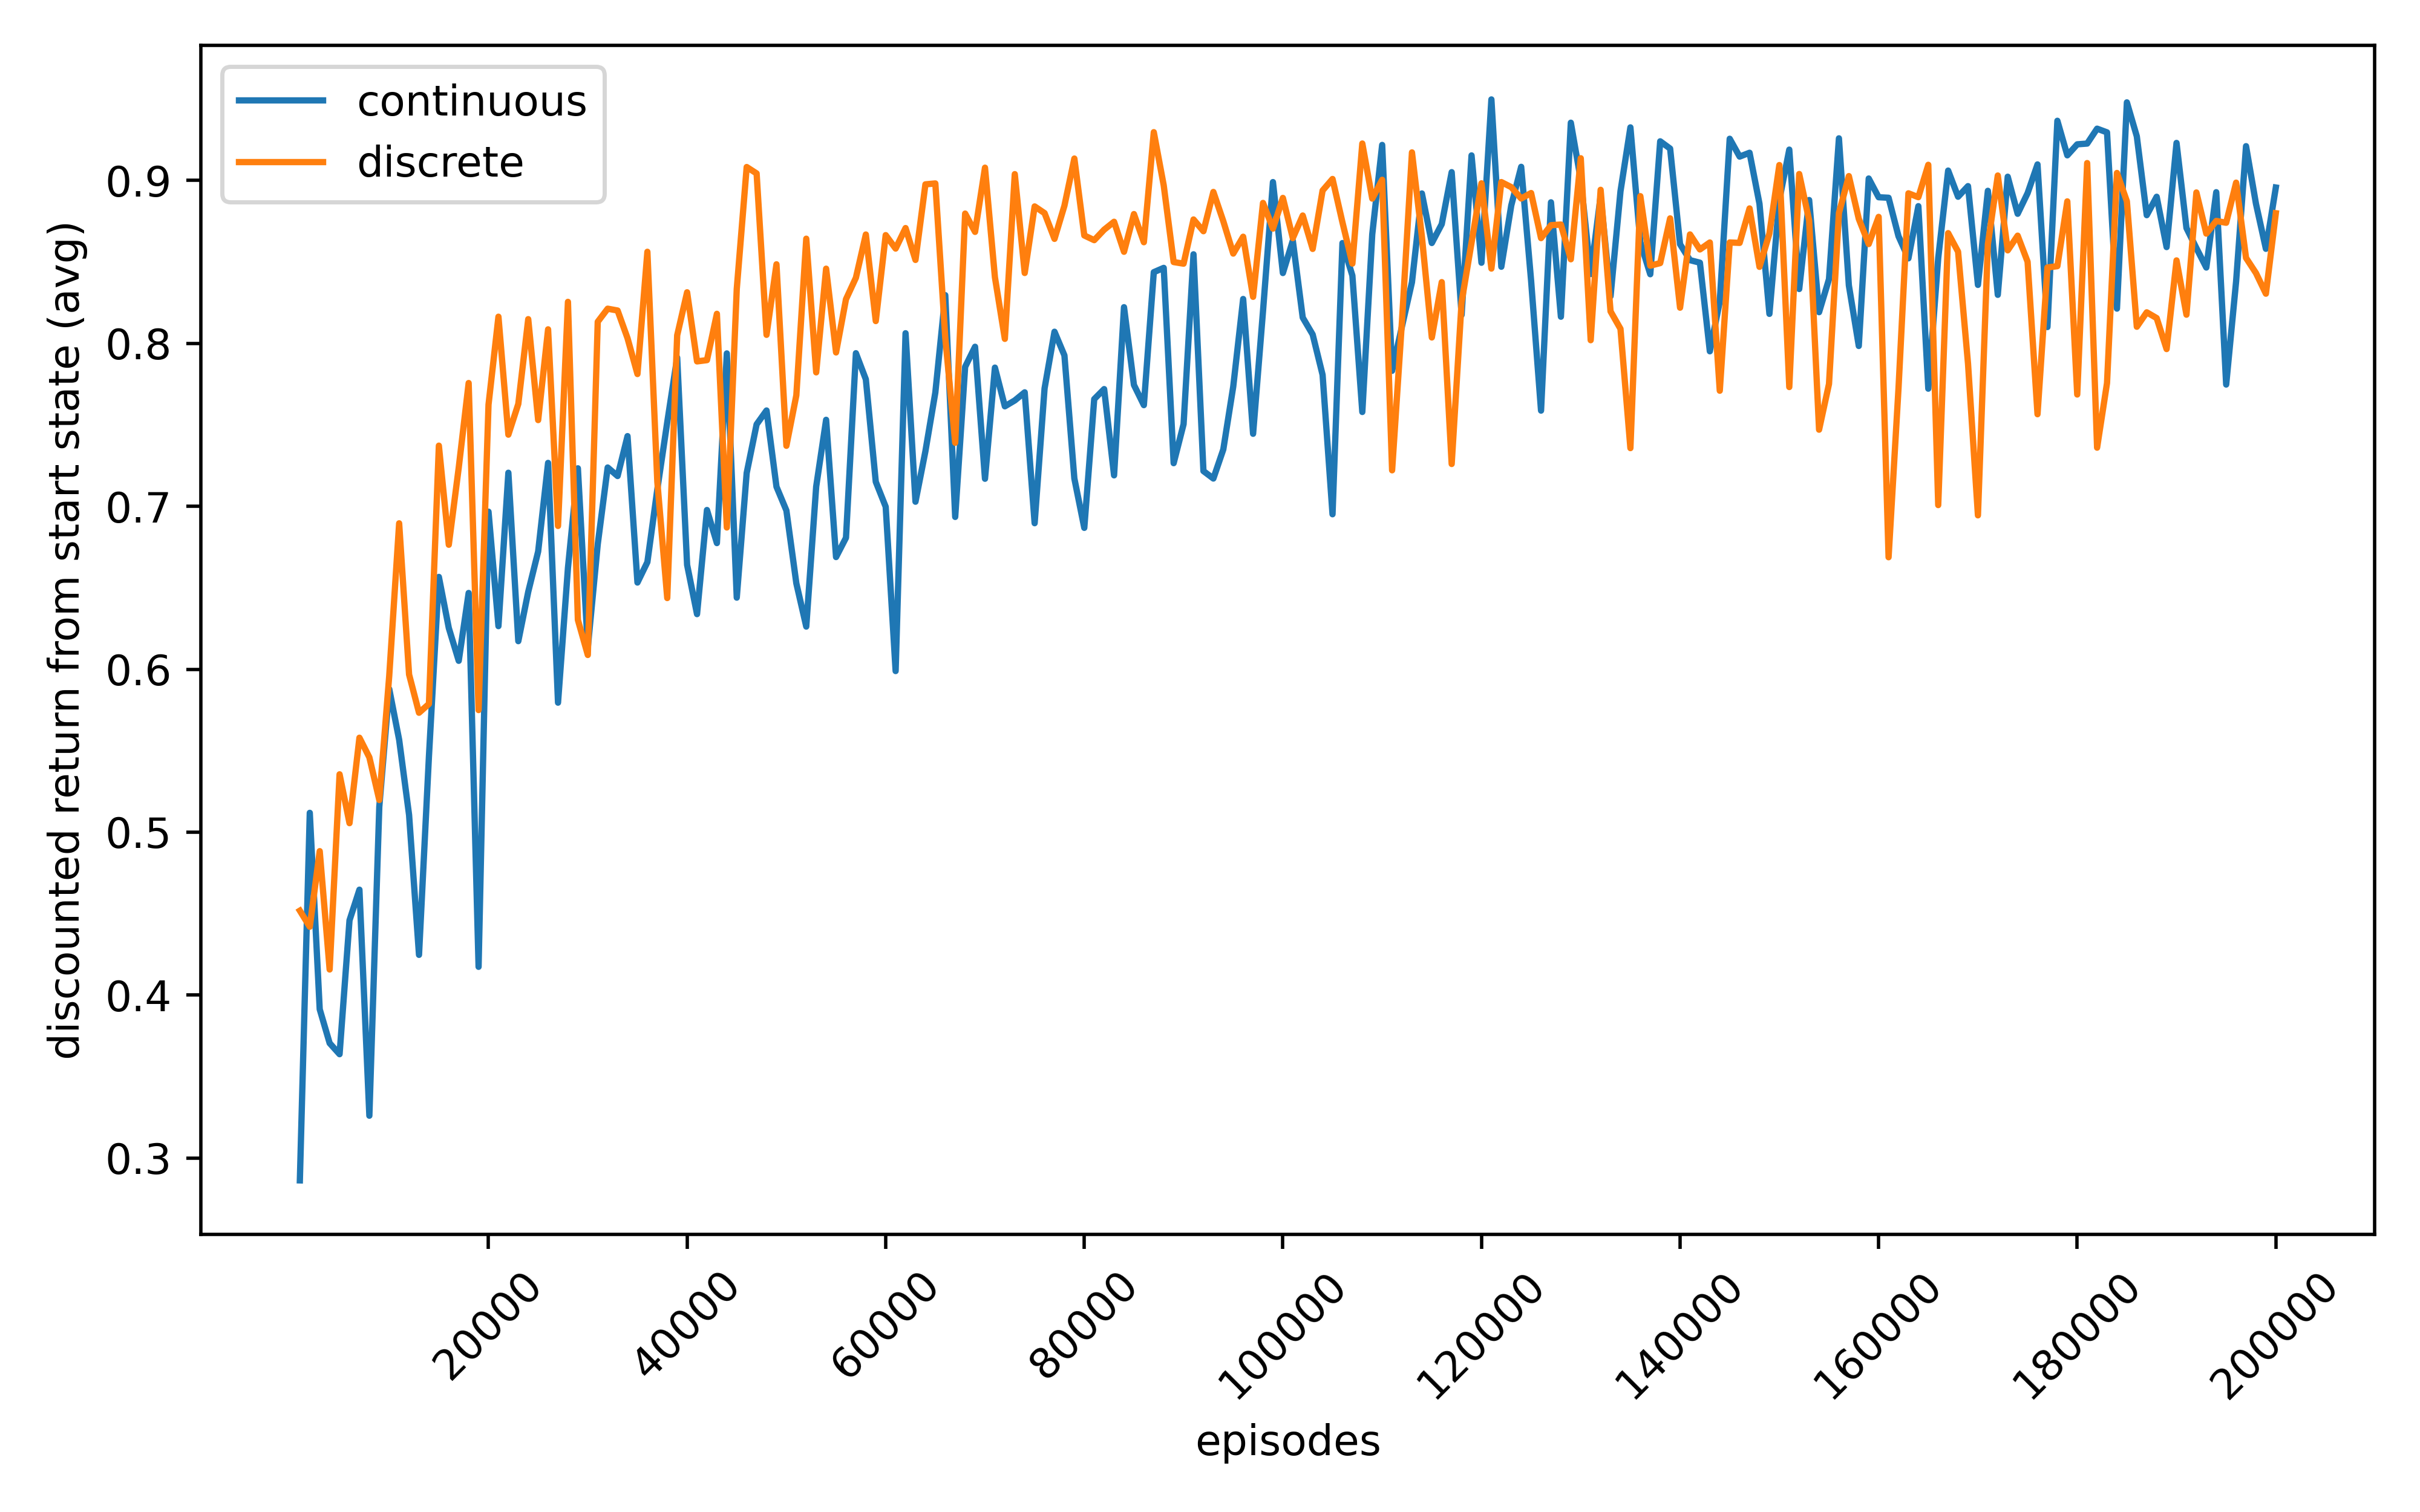
\includegraphics[width=\linewidth]{plots/part2-rewards.png}
        \caption{Discounted Return}
    \end{minipage}
    \hfill
    \begin{minipage}{0.49\linewidth}
        \centering
        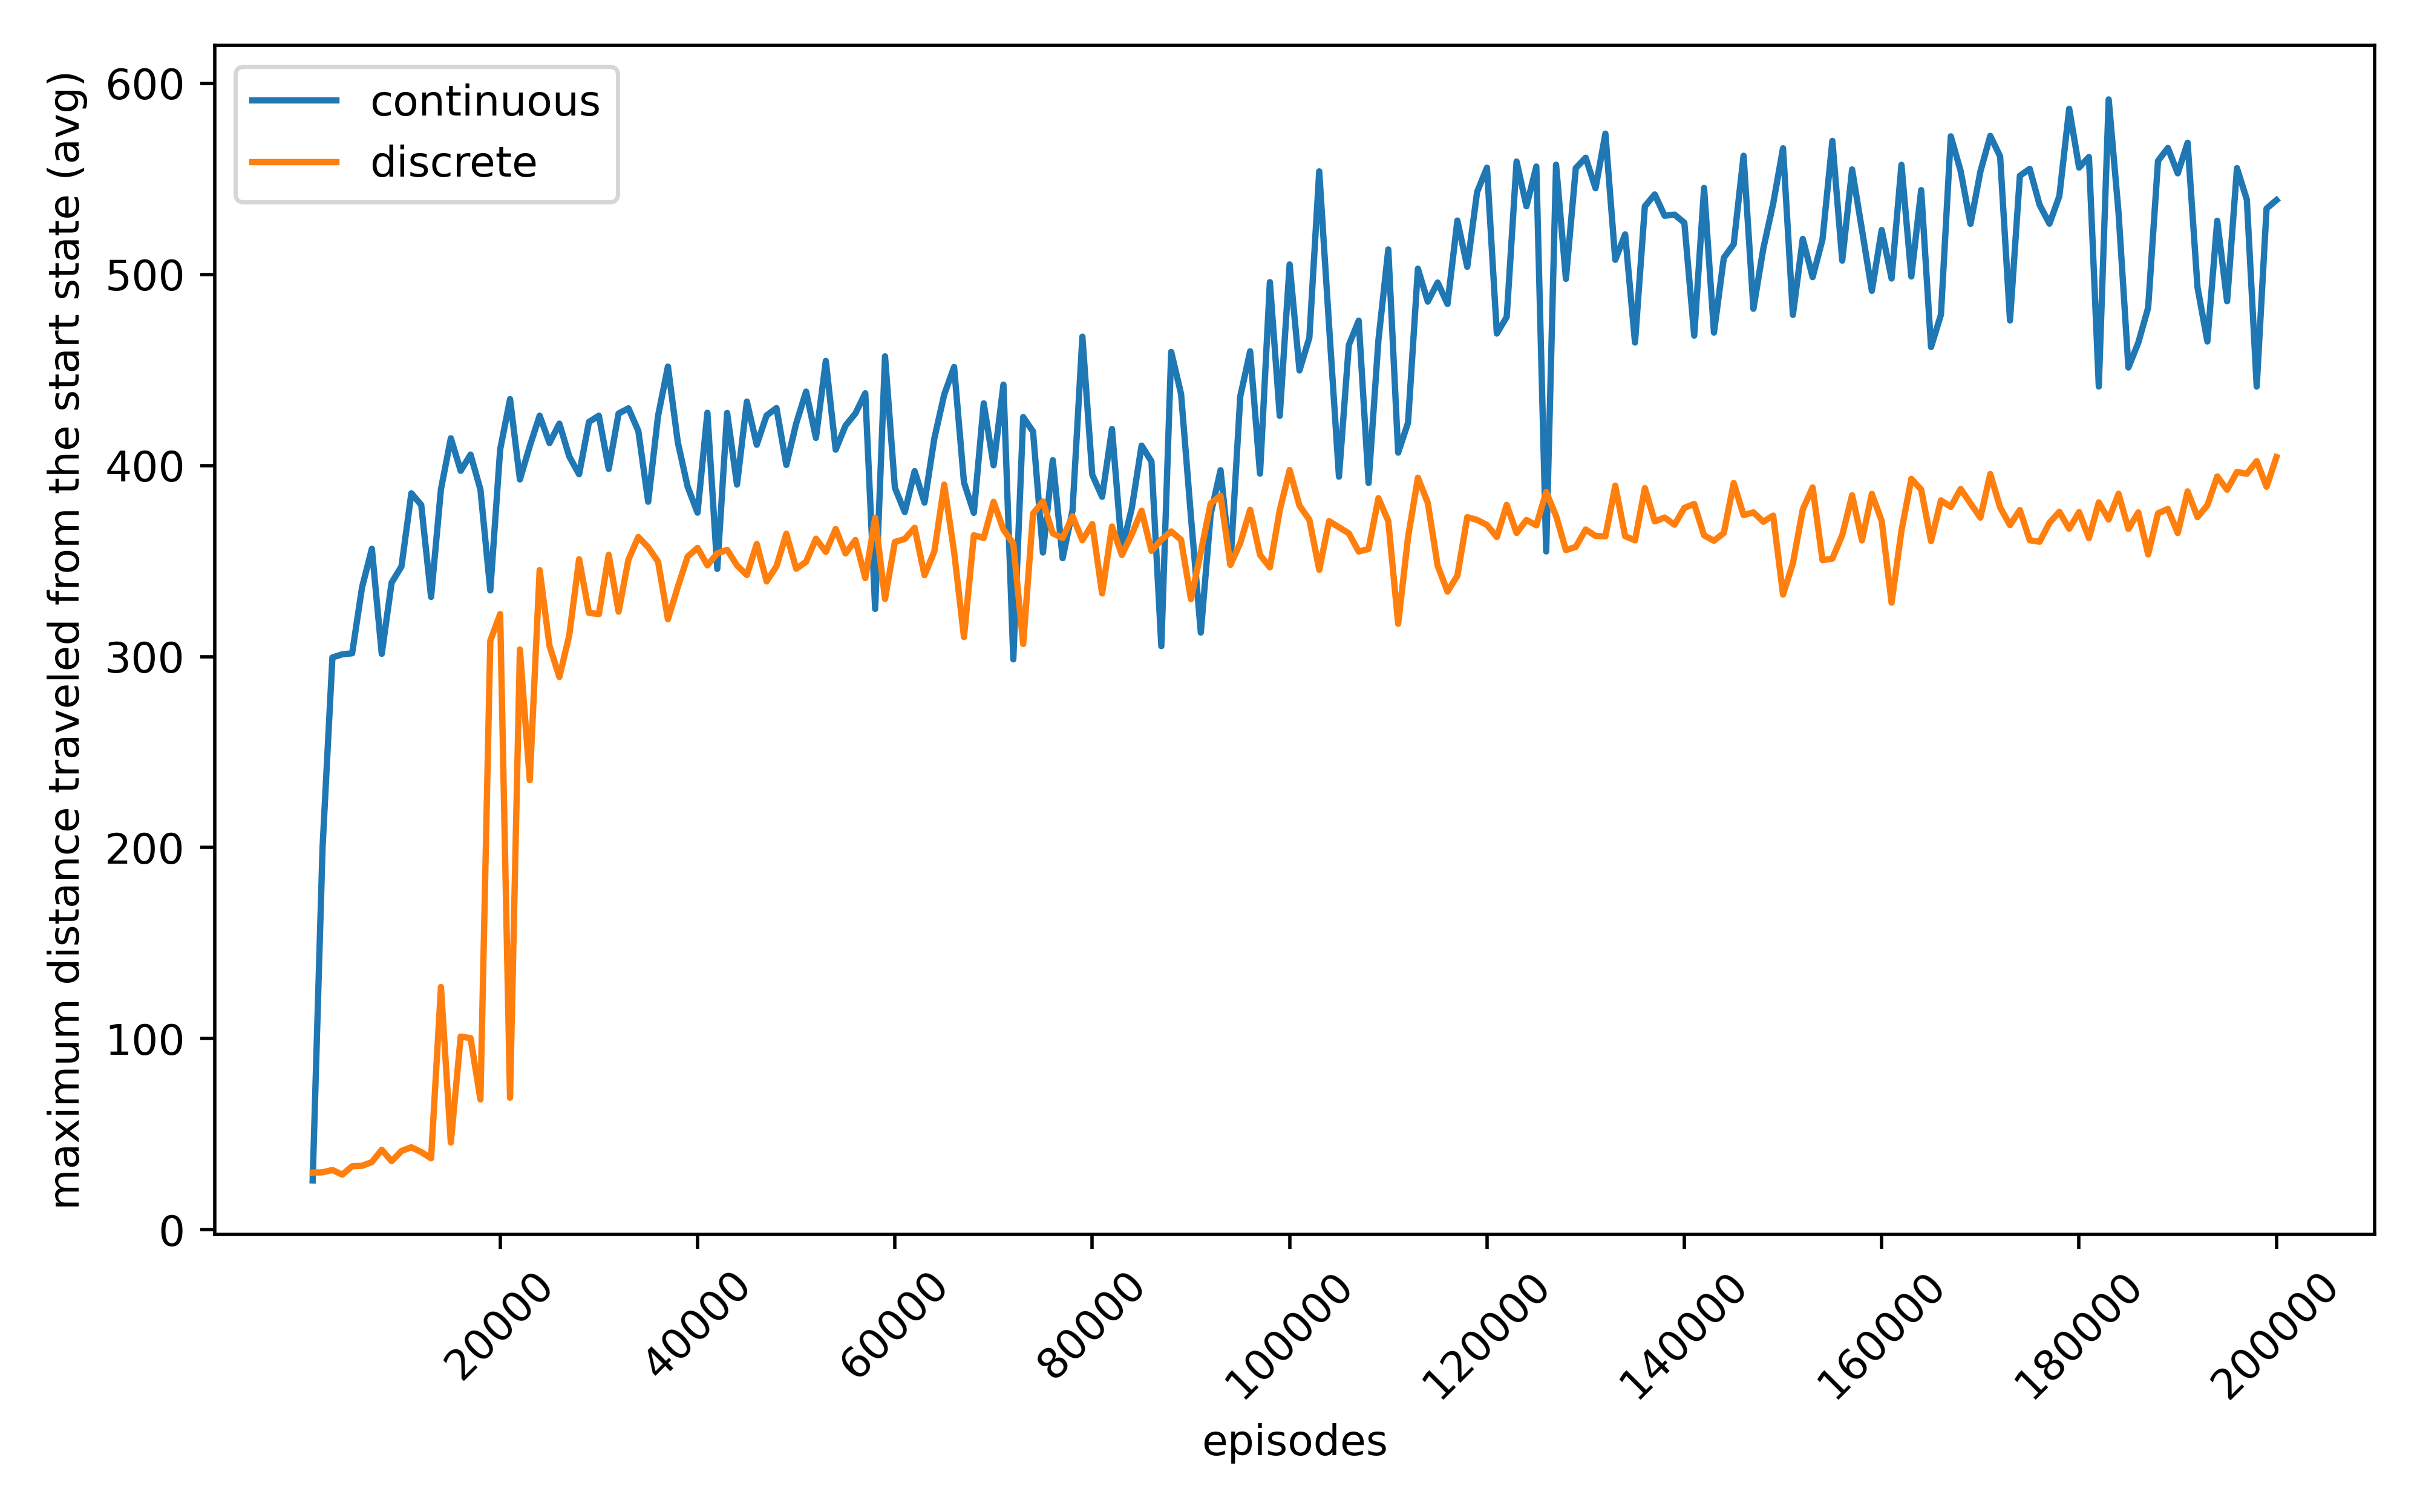
\includegraphics[width=\linewidth]{plots/part2-distances.png}
        \caption{Distance Traveled}
        \label{fig:part2-distance}
    \end{minipage}

    \vspace{1em}
    \begin{minipage}{\linewidth}
    \centering
    \begin{tabular}{lccc}
        \hline
        Model & Episodes & Discounted return & Average Distance \\
        \hline
        \texttt{Tabular} & $100,000$&$1.11$ & $531.98$ \\
        \texttt{DQN discrete}& $200,000$& $0.88$ & $404.42$ \\
        \texttt{DQN continuous} & $200,000$& $0.90$ & $538.91$ \\
        \hline
    \end{tabular}
    \caption{$\gamma = 0.9$, \texttt{Tabular} trained with $\alpha = 0.1, \epsilon = 0.75$,  \texttt{DQN} trained with \texttt{Adam} optimizer, learning rate = $10^{-4}$, batch size $256$ and replay buffer size $10,000$. For reference, maximum possible total discounted return is $1.2$.}
    \label{tab:part2}
    \end{minipage}
     \label{fig:part2}

\end{figure}
\texttt{DQN continuous} does better than \texttt{DQN discrete}. We believe this is because the $d_1, d_2, d_3, d_4$ are fed directly into the model. So the ordering, that for values of $d_1 = 0.2, 0.6, 0.9$ the order of closeness is implied. While in the discrete case, this has to be learned by the embedding layer. \texttt{DQN continuous} acts "identically" on $d_1  = 0.49$ or $d_1 = 0.51$.
\subsection{Visualization: \texttt{DQN Discrete}}
See \autoref{fig:part2.1-lane-visualization} and \autoref{fig:part2.1-speed-visualization}. The values assigned by the agent are absurd, also reflected in the low performance of the agent in \autoref{tab:part2}.


\begin{figure}[H]
    \centering
    \begin{minipage}{0.48\textwidth}
        \centering
        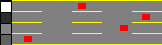
\includegraphics[width=\linewidth]{plots/part2.1-lane_visualization_00_step_0040.png}
    \end{minipage}
    \hfill
    \begin{minipage}{0.48\textwidth}
        \centering
        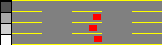
\includegraphics[width=\linewidth]{plots/part2.1-lane_visualization_00_step_0200.png}
    \end{minipage}
    \caption{Lane Visualization for \texttt{DQN Discrete} agent}
    \label{fig:part2.1-lane-visualization}
\end{figure}

\begin{figure}[H]
    \centering
    \begin{minipage}{0.48\textwidth}
        \centering
        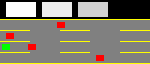
\includegraphics[width=\linewidth]{plots/part2.1-speed_visualization_00_step_0500.png}
    \end{minipage}
    \hfill
    \begin{minipage}{0.48\textwidth}
        \centering
        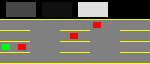
\includegraphics[width=\linewidth]{plots/part2.1-speed_visualization_00_step_0660.png}
    \end{minipage}
    \caption{Speed Visualization for    \texttt{DQN Discrete} agent}
    \label{fig:part2.1-speed-visualization}
\end{figure}


\subsection{Visualization: \texttt{DQN Continuous}}
See \autoref{fig:part2.2-lane-visualization} and \autoref{fig:part2.2-speed-visualization}. Preferences assigned are explainable, like in the Tabular-Q agent.


\begin{figure}[H]
    \centering
    \begin{minipage}{0.48\textwidth}
        \centering
        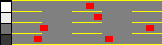
\includegraphics[width=\linewidth]{plots/part2.2-lane_visualization_00_step_0140.png}
    \end{minipage}
    \hfill
    \begin{minipage}{0.48\textwidth}
        \centering
        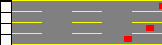
\includegraphics[width=\linewidth]{plots/part2.2-lane_visualization_00_step_0380.png}
    \end{minipage}
    \caption{Lane Visualization for \texttt{DQN Continuous} agent}
    \label{fig:part2.2-lane-visualization}
\end{figure}

\begin{figure}[H]
    \centering
    \begin{minipage}{0.48\textwidth}
        \centering
        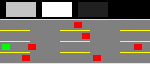
\includegraphics[width=\linewidth]{plots/part2.2-speed_visualization_00_step_0140.png}
    \end{minipage}
    \hfill
    \begin{minipage}{0.48\textwidth}
        \centering
        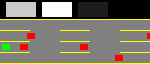
\includegraphics[width=\linewidth]{plots/part2.2-speed_visualization_01_step_0880.png}
    \end{minipage}
    \caption{Speed Visualization for    
    \texttt{DQN Continuous} agent}
    \label{fig:part2.2-speed-visualization}
\end{figure}


